\PassOptionsToPackage{unicode=true}{hyperref} % options for packages loaded elsewhere
\PassOptionsToPackage{hyphens}{url}
%
\documentclass[ignorenonframetext,]{beamer}
\usepackage{pgfpages}
\setbeamertemplate{caption}[numbered]
\setbeamertemplate{caption label separator}{: }
\setbeamercolor{caption name}{fg=normal text.fg}
\beamertemplatenavigationsymbolsempty
% Prevent slide breaks in the middle of a paragraph:
\widowpenalties 1 10000
\raggedbottom
\setbeamertemplate{part page}{
\centering
\begin{beamercolorbox}[sep=16pt,center]{part title}
  \usebeamerfont{part title}\insertpart\par
\end{beamercolorbox}
}
\setbeamertemplate{section page}{
\centering
\begin{beamercolorbox}[sep=12pt,center]{part title}
  \usebeamerfont{section title}\insertsection\par
\end{beamercolorbox}
}
\setbeamertemplate{subsection page}{
\centering
\begin{beamercolorbox}[sep=8pt,center]{part title}
  \usebeamerfont{subsection title}\insertsubsection\par
\end{beamercolorbox}
}
\AtBeginPart{
  \frame{\partpage}
}
\AtBeginSection{
  \ifbibliography
  \else
    \frame{\sectionpage}
  \fi
}
\AtBeginSubsection{
  \frame{\subsectionpage}
}
\usepackage{lmodern}
\usepackage{amssymb,amsmath}
\usepackage{ifxetex,ifluatex}
\usepackage{fixltx2e} % provides \textsubscript
\ifnum 0\ifxetex 1\fi\ifluatex 1\fi=0 % if pdftex
  \usepackage[T1]{fontenc}
  \usepackage[utf8]{inputenc}
  \usepackage{textcomp} % provides euro and other symbols
\else % if luatex or xelatex
  \usepackage{unicode-math}
  \defaultfontfeatures{Ligatures=TeX,Scale=MatchLowercase}
\fi
\usetheme[]{CambridgeUS}
\usecolortheme{beaver}
\usefonttheme{structurebold}
% use upquote if available, for straight quotes in verbatim environments
\IfFileExists{upquote.sty}{\usepackage{upquote}}{}
% use microtype if available
\IfFileExists{microtype.sty}{%
\usepackage[]{microtype}
\UseMicrotypeSet[protrusion]{basicmath} % disable protrusion for tt fonts
}{}
\IfFileExists{parskip.sty}{%
\usepackage{parskip}
}{% else
\setlength{\parindent}{0pt}
\setlength{\parskip}{6pt plus 2pt minus 1pt}
}
\usepackage{hyperref}
\hypersetup{
            pdftitle={Shapefiles},
            pdfauthor={Jan-Philipp Kolb},
            pdfborder={0 0 0},
            breaklinks=true}
\urlstyle{same}  % don't use monospace font for urls
\newif\ifbibliography
\usepackage{color}
\usepackage{fancyvrb}
\newcommand{\VerbBar}{|}
\newcommand{\VERB}{\Verb[commandchars=\\\{\}]}
\DefineVerbatimEnvironment{Highlighting}{Verbatim}{commandchars=\\\{\}}
% Add ',fontsize=\small' for more characters per line
\usepackage{framed}
\definecolor{shadecolor}{RGB}{248,248,248}
\newenvironment{Shaded}{\begin{snugshade}}{\end{snugshade}}
\newcommand{\AlertTok}[1]{\textcolor[rgb]{0.94,0.16,0.16}{#1}}
\newcommand{\AnnotationTok}[1]{\textcolor[rgb]{0.56,0.35,0.01}{\textbf{\textit{#1}}}}
\newcommand{\AttributeTok}[1]{\textcolor[rgb]{0.77,0.63,0.00}{#1}}
\newcommand{\BaseNTok}[1]{\textcolor[rgb]{0.00,0.00,0.81}{#1}}
\newcommand{\BuiltInTok}[1]{#1}
\newcommand{\CharTok}[1]{\textcolor[rgb]{0.31,0.60,0.02}{#1}}
\newcommand{\CommentTok}[1]{\textcolor[rgb]{0.56,0.35,0.01}{\textit{#1}}}
\newcommand{\CommentVarTok}[1]{\textcolor[rgb]{0.56,0.35,0.01}{\textbf{\textit{#1}}}}
\newcommand{\ConstantTok}[1]{\textcolor[rgb]{0.00,0.00,0.00}{#1}}
\newcommand{\ControlFlowTok}[1]{\textcolor[rgb]{0.13,0.29,0.53}{\textbf{#1}}}
\newcommand{\DataTypeTok}[1]{\textcolor[rgb]{0.13,0.29,0.53}{#1}}
\newcommand{\DecValTok}[1]{\textcolor[rgb]{0.00,0.00,0.81}{#1}}
\newcommand{\DocumentationTok}[1]{\textcolor[rgb]{0.56,0.35,0.01}{\textbf{\textit{#1}}}}
\newcommand{\ErrorTok}[1]{\textcolor[rgb]{0.64,0.00,0.00}{\textbf{#1}}}
\newcommand{\ExtensionTok}[1]{#1}
\newcommand{\FloatTok}[1]{\textcolor[rgb]{0.00,0.00,0.81}{#1}}
\newcommand{\FunctionTok}[1]{\textcolor[rgb]{0.00,0.00,0.00}{#1}}
\newcommand{\ImportTok}[1]{#1}
\newcommand{\InformationTok}[1]{\textcolor[rgb]{0.56,0.35,0.01}{\textbf{\textit{#1}}}}
\newcommand{\KeywordTok}[1]{\textcolor[rgb]{0.13,0.29,0.53}{\textbf{#1}}}
\newcommand{\NormalTok}[1]{#1}
\newcommand{\OperatorTok}[1]{\textcolor[rgb]{0.81,0.36,0.00}{\textbf{#1}}}
\newcommand{\OtherTok}[1]{\textcolor[rgb]{0.56,0.35,0.01}{#1}}
\newcommand{\PreprocessorTok}[1]{\textcolor[rgb]{0.56,0.35,0.01}{\textit{#1}}}
\newcommand{\RegionMarkerTok}[1]{#1}
\newcommand{\SpecialCharTok}[1]{\textcolor[rgb]{0.00,0.00,0.00}{#1}}
\newcommand{\SpecialStringTok}[1]{\textcolor[rgb]{0.31,0.60,0.02}{#1}}
\newcommand{\StringTok}[1]{\textcolor[rgb]{0.31,0.60,0.02}{#1}}
\newcommand{\VariableTok}[1]{\textcolor[rgb]{0.00,0.00,0.00}{#1}}
\newcommand{\VerbatimStringTok}[1]{\textcolor[rgb]{0.31,0.60,0.02}{#1}}
\newcommand{\WarningTok}[1]{\textcolor[rgb]{0.56,0.35,0.01}{\textbf{\textit{#1}}}}
\usepackage{longtable,booktabs}
\usepackage{caption}
% These lines are needed to make table captions work with longtable:
\makeatletter
\def\fnum@table{\tablename~\thetable}
\makeatother
\usepackage{graphicx,grffile}
\makeatletter
\def\maxwidth{\ifdim\Gin@nat@width>\linewidth\linewidth\else\Gin@nat@width\fi}
\def\maxheight{\ifdim\Gin@nat@height>\textheight\textheight\else\Gin@nat@height\fi}
\makeatother
% Scale images if necessary, so that they will not overflow the page
% margins by default, and it is still possible to overwrite the defaults
% using explicit options in \includegraphics[width, height, ...]{}
\setkeys{Gin}{width=\maxwidth,height=\maxheight,keepaspectratio}
\setlength{\emergencystretch}{3em}  % prevent overfull lines
\providecommand{\tightlist}{%
  \setlength{\itemsep}{0pt}\setlength{\parskip}{0pt}}
\setcounter{secnumdepth}{0}

% set default figure placement to htbp
\makeatletter
\def\fps@figure{htbp}
\makeatother


\title{Shapefiles}
\author{Jan-Philipp Kolb}
\date{22 Oktober 2018}

\begin{document}
\frame{\titlepage}

\begin{frame}[fragile]{Worum geht es in diesem Abschnitt}
\protect\hypertarget{worum-geht-es-in-diesem-abschnitt}{}

\begin{itemize}
\tightlist
\item
  Was sind Shapefiles?
\item
  Wie kann man Shapefiles (\texttt{.shp}) in R importieren?
\item
  Der Import von Shapefiles wird anhand von Vorwahl- und PLZ-Bereichen
  gezeigt.
\item
  Wie kann man einzelne Polygonzüge zusammenfassen?
\end{itemize}

\end{frame}

\begin{frame}{Ein kleines Quizz}
\protect\hypertarget{ein-kleines-quizz}{}

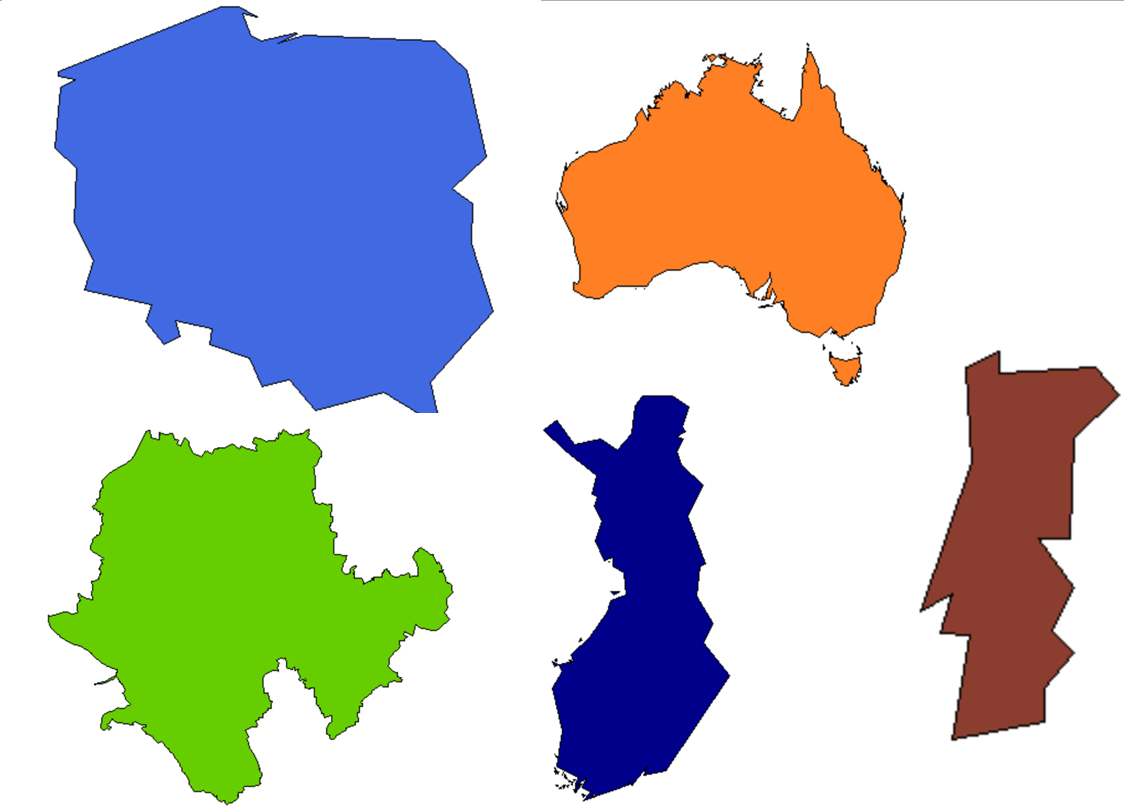
\includegraphics{D:/GitHub/IntroR/buildingblocks/figure/quizz.PNG}

\end{frame}

\begin{frame}{Das shapefile Format \ldots{}}
\protect\hypertarget{das-shapefile-format}{}

\begin{itemize}
\item
  \ldots{} ist ein beliebtes Format räumlicher Vektordaten für
  geographisches Informationssysteme (GIS).
\item
  Das Dateiformat Shapefile ist ein ursprünglich für die Software
  ArcView der Firma ESRI entwickeltes Format für Geodaten. (Quelle:
  \href{https://de.wikipedia.org/wiki/Shapefile}{\textbf{Wikipedia}})
\item
  Es wurde entwickelt und reguliert von
  \href{http://www.esri.com/}{\textbf{ESRI}}
\item
  (meist) offene Spezifikation um Daten Interoperabilität zwischen Esri
  und anderen Formaten zu sichern.
\item
  Es können Punkte, Linien und Polygone beschrieben werden
\item
  Jedes Element hat Attribute, wie bspw. Name oder Temperatur die es
  beschreiben.
\end{itemize}

Quelle: \url{https://en.wikipedia.org/wiki/Shapefile}

\end{frame}

\begin{frame}{Der R Befehl readShapePoly}
\protect\hypertarget{der-r-befehl-readshapepoly}{}

Um Shape-Dateien zu lesen, ist es notwendig, die drei Dateien mit den
folgenden Dateierweiterungen im gleichen Verzeichnis zu haben:

\begin{itemize}
\tightlist
\item
  .shp
\item
  .dbf
\item
  .shx
\end{itemize}

\end{frame}

\begin{frame}[fragile]{\href{http://www.bundesnetzagentur.de/SharedDocs/Downloads/DE/Sachgebiete/Telekommunikation/Unternehmen_Institutionen/Nummerierung/Rufnummern/ONVerzeichnisse/ONBGrenzen/ONB_Grenzen.html}{\textbf{Vorwahlbereiche
in Deutschland}}}
\protect\hypertarget{vorwahlbereiche-in-deutschland}{}

\begin{block}{Quelle Ortsnetzbereiche:
\href{https://www.bundesnetzagentur.de/DE/Sachgebiete/Telekommunikation/Unternehmen_Institutionen/Nummerierung/Rufnummern/ONRufnr/ON_Einteilung_ONB/ON_ONB_ONKz_ONBGrenzen_Basepage.html}{\textbf{Bundesnetzagentur}}}

\begin{itemize}
\item
  \href{https://www.bundesnetzagentur.de/SharedDocs/Downloads/DE/Sachgebiete/Telekommunikation/Unternehmen_Institutionen/Nummerierung/Rufnummern/ONVerzeichnisse/ONBGrenzen/ONB-Grenzen-2018.zip?__blob=publicationFile\&v=21}{\textbf{Download}}
  ONB-Grenzen
\item
  Wir verwenden das Paket \texttt{maptools} um die Daten einzulesen:
\end{itemize}

\begin{Shaded}
\begin{Highlighting}[]
\KeywordTok{setwd}\NormalTok{(geodata_path)}
\KeywordTok{library}\NormalTok{(maptools)}
\NormalTok{onb <-}\StringTok{ }\KeywordTok{readShapePoly}\NormalTok{(}\StringTok{"onb_grenzen.shp"}\NormalTok{)}
\end{Highlighting}
\end{Shaded}

\end{block}

\end{frame}

\begin{frame}[fragile]{Die Karte zeichnen}
\protect\hypertarget{die-karte-zeichnen}{}

\begin{Shaded}
\begin{Highlighting}[]
\KeywordTok{plot}\NormalTok{(onb)}
\end{Highlighting}
\end{Shaded}

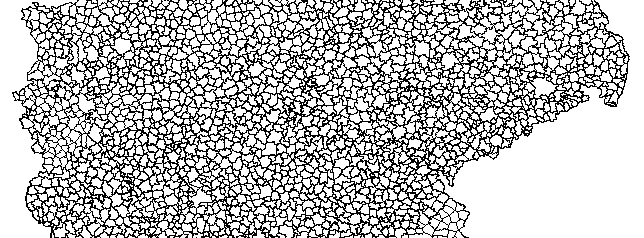
\includegraphics{D:/GitHub/IntroR/buildingblocks/figure/ONB_bereiche.PNG}

\end{frame}

\begin{frame}[fragile]{Der Datenslot}
\protect\hypertarget{der-datenslot}{}

\begin{Shaded}
\begin{Highlighting}[]
\KeywordTok{kable}\NormalTok{(}\KeywordTok{head}\NormalTok{(onb}\OperatorTok{@}\NormalTok{data))}
\end{Highlighting}
\end{Shaded}

\begin{longtable}[]{@{}llll@{}}
\toprule
& VORWAHL & NAME & KENNUNG\tabularnewline
\midrule
\endhead
0 & 04651 & Sylt & NA\tabularnewline
1 & 04668 & Klanxbüll & NA\tabularnewline
2 & 04664 & Neukirchen b Niebüll & NA\tabularnewline
3 & 04663 & Süderlügum & NA\tabularnewline
4 & 04666 & Ladelund & NA\tabularnewline
5 & 04631 & Glücksburg Ostsee & NA\tabularnewline
\bottomrule
\end{longtable}

\end{frame}

\begin{frame}[fragile]{Einen Vorwahlbereich ausschneiden}
\protect\hypertarget{einen-vorwahlbereich-ausschneiden}{}

\begin{Shaded}
\begin{Highlighting}[]
\NormalTok{vwb <-}\StringTok{ }\NormalTok{onb}\OperatorTok{@}\NormalTok{data}\OperatorTok{$}\NormalTok{VORWAHL}
\NormalTok{vwb2 <-}\StringTok{ }\KeywordTok{substr}\NormalTok{(vwb, }\DecValTok{1}\NormalTok{,}\DecValTok{2}\NormalTok{)}
\end{Highlighting}
\end{Shaded}

\begin{Shaded}
\begin{Highlighting}[]
\KeywordTok{library}\NormalTok{(lattice)}
\KeywordTok{barchart}\NormalTok{(}\KeywordTok{table}\NormalTok{(vwb2),}\DataTypeTok{col=}\StringTok{"royalblue"}\NormalTok{,}
         \DataTypeTok{xlab=}\StringTok{"Häufigkeit"}\NormalTok{)}
\end{Highlighting}
\end{Shaded}

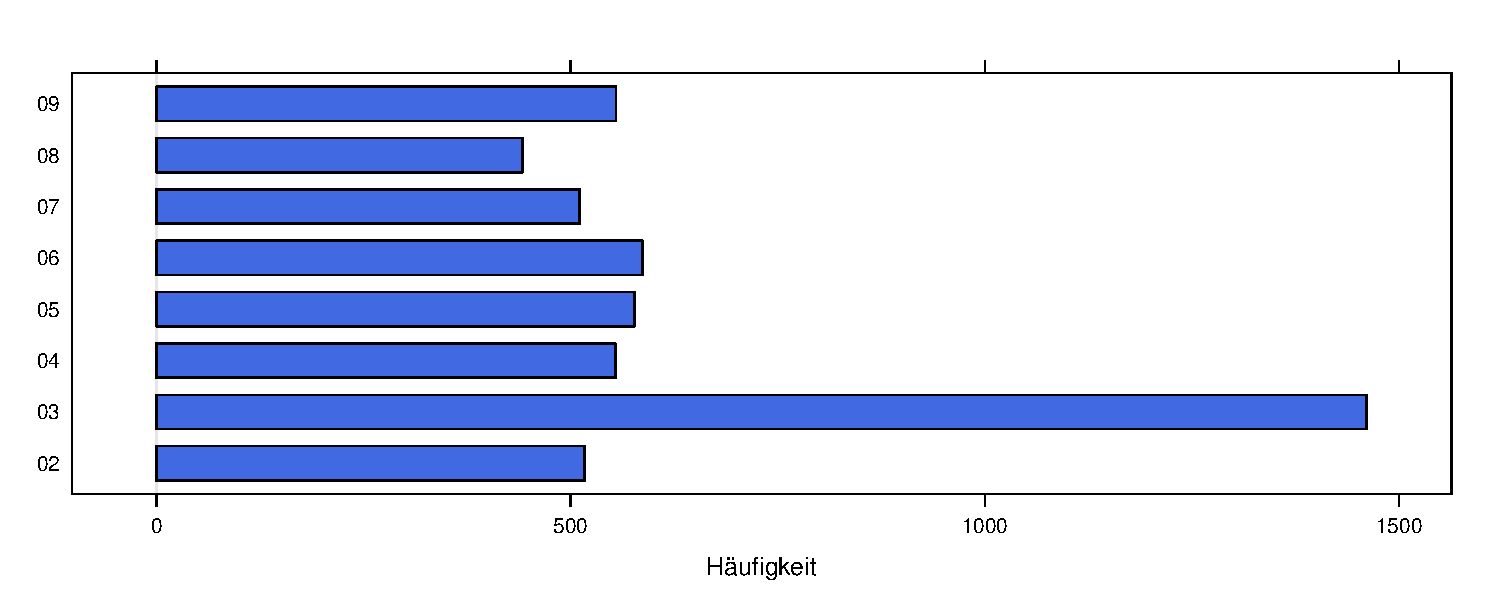
\includegraphics{shapefiles_files/figure-beamer/unnamed-chunk-11-1.pdf}

\end{frame}

\begin{frame}[fragile]{Vorwahlbereich ausschneiden}
\protect\hypertarget{vorwahlbereich-ausschneiden}{}

\begin{Shaded}
\begin{Highlighting}[]
\NormalTok{vwb6 <-}\StringTok{ }\NormalTok{onb[vwb2}\OperatorTok{==}\StringTok{"06"}\NormalTok{,]}
\KeywordTok{plot}\NormalTok{(vwb6)}
\end{Highlighting}
\end{Shaded}


\includegraphics{shapefiles_files/figure-beamer/unnamed-chunk-12-1.pdf}

\end{frame}

\begin{frame}[fragile]{Shapefiles zusammenfassen}
\protect\hypertarget{shapefiles-zusammenfassen}{}

\begin{Shaded}
\begin{Highlighting}[]
\NormalTok{vwb6c <-}\StringTok{ }\KeywordTok{unionSpatialPolygons}\NormalTok{(vwb6,}
              \KeywordTok{rep}\NormalTok{(}\DecValTok{1}\NormalTok{,}\KeywordTok{length}\NormalTok{(vwb6)))}
\KeywordTok{plot}\NormalTok{(vwb6c,}\DataTypeTok{col=}\StringTok{"royalblue"}\NormalTok{)}
\end{Highlighting}
\end{Shaded}


\includegraphics{shapefiles_files/figure-beamer/unnamed-chunk-13-1.pdf}

\end{frame}

\begin{frame}[fragile]{Wo ist Mannheim?}
\protect\hypertarget{wo-ist-mannheim}{}

\begin{Shaded}
\begin{Highlighting}[]
\NormalTok{Com <-}\StringTok{ }\NormalTok{vwb6}\OperatorTok{@}\NormalTok{data}\OperatorTok{$}\NormalTok{NAME}
\KeywordTok{plot}\NormalTok{(vwb6)}
\KeywordTok{plot}\NormalTok{(vwb6[Com}\OperatorTok{==}\StringTok{"Mannheim"}\NormalTok{,],}\DataTypeTok{col=}\StringTok{"red"}\NormalTok{,}\DataTypeTok{add=}\NormalTok{T)}
\KeywordTok{plot}\NormalTok{(vwb6[Com}\OperatorTok{==}\StringTok{"Heidelberg"}\NormalTok{,],}\DataTypeTok{col=}\StringTok{"green"}\NormalTok{,}\DataTypeTok{add=}\NormalTok{T)}
\KeywordTok{plot}\NormalTok{(vwb6[Com}\OperatorTok{==}\StringTok{"Kaiserslautern"}\NormalTok{,],}\DataTypeTok{col=}\StringTok{"blue"}\NormalTok{,}\DataTypeTok{add=}\NormalTok{T)}
\end{Highlighting}
\end{Shaded}


\includegraphics{shapefiles_files/figure-beamer/unnamed-chunk-14-1.pdf}

\end{frame}

\begin{frame}{Shapefiles für PLZ-Bereiche}
\protect\hypertarget{shapefiles-fur-plz-bereiche}{}

\begin{block}{\href{http://arnulf.us/PLZ}{\textbf{Quelle}} für PLZ
Shapefiles}

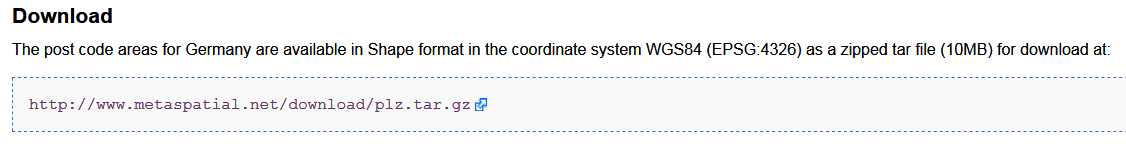
\includegraphics{D:/GitHub/IntroR/buildingblocks/figure/Download_plz.PNG}

\end{block}

\end{frame}

\begin{frame}[fragile]{Paket \texttt{rgdal} - PLZ Datensatz einlesen}
\protect\hypertarget{paket-rgdal---plz-datensatz-einlesen}{}

\begin{Shaded}
\begin{Highlighting}[]
\KeywordTok{library}\NormalTok{(rgdal)}
\end{Highlighting}
\end{Shaded}

\begin{Shaded}
\begin{Highlighting}[]
\KeywordTok{setwd}\NormalTok{(data_path)}
\NormalTok{plz <-}\StringTok{ }\KeywordTok{readOGR}\NormalTok{ (}\StringTok{"post_pl.shp"}\NormalTok{,}\StringTok{"post_pl"}\NormalTok{)}
\end{Highlighting}
\end{Shaded}

\begin{verbatim}
## OGR data source with driver: ESRI Shapefile 
## Source: "D:\GESIS\data\post_pl.shp", layer: "post_pl"
## with 8270 features
## It has 3 fields
\end{verbatim}

\end{frame}

\begin{frame}[fragile]{Die Daten plotten}
\protect\hypertarget{die-daten-plotten}{}

\begin{Shaded}
\begin{Highlighting}[]
\NormalTok{plzbereich <-}\StringTok{ }\KeywordTok{substr}\NormalTok{(plz}\OperatorTok{@}\NormalTok{data}\OperatorTok{$}\NormalTok{PLZ99,}\DecValTok{1}\NormalTok{,}\DecValTok{2}\NormalTok{)}
\KeywordTok{plot}\NormalTok{(plz[plzbereich}\OperatorTok{==}\StringTok{"68"}\NormalTok{,])}
\end{Highlighting}
\end{Shaded}


\includegraphics{shapefiles_files/figure-beamer/unnamed-chunk-19-1.pdf}

\end{frame}

\begin{frame}[fragile]{Die Grenze von Mannheim}
\protect\hypertarget{die-grenze-von-mannheim}{}

\begin{Shaded}
\begin{Highlighting}[]
\NormalTok{ma_map <-}\StringTok{ }\NormalTok{plz[plz}\OperatorTok{$}\NormalTok{PLZORT99}\OperatorTok{==}\StringTok{"Mannheim"}\NormalTok{,]}
\KeywordTok{plot}\NormalTok{(ma_map)}
\end{Highlighting}
\end{Shaded}


\includegraphics{shapefiles_files/figure-beamer/unnamed-chunk-20-1.pdf}

\end{frame}

\begin{frame}[fragile]{Die PLZ-Bereiche von Mannheim zusammenfassen}
\protect\hypertarget{die-plz-bereiche-von-mannheim-zusammenfassen}{}

\begin{itemize}
\tightlist
\item
  Wir nutzen den Befehl \texttt{unionSpatialPolygons} im Paket
  \texttt{maptools}
\end{itemize}

\begin{Shaded}
\begin{Highlighting}[]
\KeywordTok{library}\NormalTok{(maptools)}
\NormalTok{ma_map2 <-}\StringTok{ }\KeywordTok{unionSpatialPolygons}\NormalTok{(}\DataTypeTok{SpP =}\NormalTok{ ma_map,}
                                \DataTypeTok{IDs =} \KeywordTok{rep}\NormalTok{(}\DecValTok{1}\NormalTok{,}\KeywordTok{length}\NormalTok{(ma_map)))}
\KeywordTok{plot}\NormalTok{(ma_map2)}
\end{Highlighting}
\end{Shaded}


\includegraphics{shapefiles_files/figure-beamer/unnamed-chunk-21-1.pdf}

\end{frame}

\begin{frame}[fragile]{Exkurs: der Befehl \texttt{agrep}}
\protect\hypertarget{exkurs-der-befehl-agrep}{}

\begin{Shaded}
\begin{Highlighting}[]
\KeywordTok{agrep}\NormalTok{(}\StringTok{"Freiburg"}\NormalTok{,plz}\OperatorTok{@}\NormalTok{data}\OperatorTok{$}\NormalTok{PLZORT99)}
\end{Highlighting}
\end{Shaded}

\begin{verbatim}
##  [1]  363  660  661 1349 5074 5798 5799 5800 5801 5802 5803 5804 5805 5806
## [15] 5807 5808 5809
\end{verbatim}

\begin{Shaded}
\begin{Highlighting}[]
\KeywordTok{agrep}\NormalTok{(}\StringTok{"Freiburg"}\NormalTok{,plz}\OperatorTok{@}\NormalTok{data}\OperatorTok{$}\NormalTok{PLZORT99,}\DataTypeTok{value=}\NormalTok{T)}
\end{Highlighting}
\end{Shaded}

\begin{verbatim}
##  [1] "Freyburg/ Unstrut"    "Freiberg"             "Freiberg"            
##  [4] "Freiburg (Elbe)"      "Freiberg am Neckar"   "Freiburg im Breisgau"
##  [7] "Freiburg im Breisgau" "Freiburg im Breisgau" "Freiburg im Breisgau"
## [10] "Freiburg im Breisgau" "Freiburg im Breisgau" "Freiburg im Breisgau"
## [13] "Freiburg im Breisgau" "Freiburg im Breisgau" "Freiburg im Breisgau"
## [16] "Freiburg im Breisgau" "Freiburg im Breisgau"
\end{verbatim}

\end{frame}

\begin{frame}[fragile]{Die Funktion \texttt{grep}}
\protect\hypertarget{die-funktion-grep}{}

\begin{block}{Der exakte match}

\begin{Shaded}
\begin{Highlighting}[]
\KeywordTok{grep}\NormalTok{(}\StringTok{"Freiburg"}\NormalTok{,plz}\OperatorTok{@}\NormalTok{data}\OperatorTok{$}\NormalTok{PLZORT99,}\DataTypeTok{value=}\NormalTok{T)}
\end{Highlighting}
\end{Shaded}

\begin{verbatim}
##  [1] "Freiburg (Elbe)"      "Freiburg im Breisgau" "Freiburg im Breisgau"
##  [4] "Freiburg im Breisgau" "Freiburg im Breisgau" "Freiburg im Breisgau"
##  [7] "Freiburg im Breisgau" "Freiburg im Breisgau" "Freiburg im Breisgau"
## [10] "Freiburg im Breisgau" "Freiburg im Breisgau" "Freiburg im Breisgau"
## [13] "Freiburg im Breisgau"
\end{verbatim}

\begin{Shaded}
\begin{Highlighting}[]
\KeywordTok{agrep}\NormalTok{(}\StringTok{"Freiburg"}\NormalTok{,plz}\OperatorTok{@}\NormalTok{data}\OperatorTok{$}\NormalTok{PLZORT99,}\DataTypeTok{value=}\NormalTok{T,}
      \DataTypeTok{max.distance =} \FloatTok{0.2}\NormalTok{)}
\end{Highlighting}
\end{Shaded}

\begin{verbatim}
##  [1] "Frohburg"             "Freyburg/ Unstrut"    "Freiberg"            
##  [4] "Freiberg"             "Freiburg (Elbe)"      "Ehrenburg"           
##  [7] "Gnarrenburg"          "Bad Driburg"          "Derenburg"           
## [10] "Freiberg am Neckar"   "Freiburg im Breisgau" "Freiburg im Breisgau"
## [13] "Freiburg im Breisgau" "Freiburg im Breisgau" "Freiburg im Breisgau"
## [16] "Freiburg im Breisgau" "Freiburg im Breisgau" "Freiburg im Breisgau"
## [19] "Freiburg im Breisgau" "Freiburg im Breisgau" "Freiburg im Breisgau"
## [22] "Freiburg im Breisgau" "Waldkraiburg"         "Kraiburg a. Inn"     
## [25] "Freihung"
\end{verbatim}

\end{block}

\end{frame}

\begin{frame}[fragile]{A6A Übung - PLZ Bereiche herunterladen}
\protect\hypertarget{a6a-ubung---plz-bereiche-herunterladen}{}

\begin{itemize}
\tightlist
\item
  Lade den Shapefile mit den PLZ-Bereichen
  \href{http://arnulf.us/PLZ}{\textbf{hier}} herunter.
\item
  Importiere den Shapefile in R mit einem geeigneten Befehl.
\item
  Erzeuge einen Datensatz mit den PLZ-Bereichen von Berlin.
\item
  Speichere den Datensatz als \texttt{.RData} Datei ab.
\end{itemize}

\end{frame}

\begin{frame}[fragile]{Global Adminastrative Boundaries -
\href{http://www.gadm.org/}{GADM} - NUTS level 1}
\protect\hypertarget{global-adminastrative-boundaries---gadm---nuts-level-1}{}

\begin{itemize}
\tightlist
\item
  Für Polygonzüge unterhalb der Staatsgrenzen ist
  \href{http://www.gadm.org/}{\textbf{Global Administrative Boundaries}}
  eine gute Quelle.
\item
  Vor allem wegen API, die man Paket \texttt{raster} nutzen kann.
\end{itemize}

\begin{Shaded}
\begin{Highlighting}[]
\KeywordTok{library}\NormalTok{(raster)}
\NormalTok{LUX1 <-}\StringTok{ }\KeywordTok{getData}\NormalTok{(}\StringTok{'GADM'}\NormalTok{, }\DataTypeTok{country=}\StringTok{'LUX'}\NormalTok{, }\DataTypeTok{level=}\DecValTok{1}\NormalTok{)}
\KeywordTok{plot}\NormalTok{(LUX1)}
\end{Highlighting}
\end{Shaded}


\includegraphics{shapefiles_files/figure-beamer/unnamed-chunk-28-1.pdf}

\end{frame}

\begin{frame}[fragile]{Ein Blick auf die Daten}
\protect\hypertarget{ein-blick-auf-die-daten}{}

Koordinaten im polygon slot

\begin{Shaded}
\begin{Highlighting}[]
\NormalTok{LUX1}\OperatorTok{@}\NormalTok{polygons[[}\DecValTok{1}\NormalTok{]]}\OperatorTok{@}\NormalTok{Polygons[[}\DecValTok{1}\NormalTok{]]}\OperatorTok{@}\NormalTok{coords}
\end{Highlighting}
\end{Shaded}

\begin{verbatim}
##             x        y
## [1,] 6.238343 49.78491
## [2,] 6.238727 49.78969
## [3,] 6.238657 49.79102
## [4,] 6.238348 49.79232
## [5,] 6.238039 49.79295
## [6,] 6.237128 49.79403
\end{verbatim}

\end{frame}

\begin{frame}[fragile]{Der Datenslot}
\protect\hypertarget{der-datenslot-1}{}

\begin{Shaded}
\begin{Highlighting}[]
\KeywordTok{head}\NormalTok{(LUX1}\OperatorTok{@}\NormalTok{data)}
\end{Highlighting}
\end{Shaded}

\begin{verbatim}
##   GID_0     NAME_0   GID_1       NAME_1            VARNAME_1 NL_NAME_1
## 1   LUX Luxembourg LUX.1_1     Diekirch     Dikrech|Dikkrich      <NA>
## 2   LUX Luxembourg LUX.2_1 Grevenmacher        Gréivemaacher      <NA>
## 3   LUX Luxembourg LUX.3_1   Luxembourg Lëtzebuerg|Luxemburg      <NA>
##     TYPE_1 ENGTYPE_1 CC_1 HASC_1
## 1 District  District <NA>  LU.DI
## 2 District  District <NA>  LU.GR
## 3 District  District <NA>  LU.LU
\end{verbatim}

\end{frame}

\begin{frame}[fragile]{\href{http://www.gadm.org/}{GADM}- NUTS level 3}
\protect\hypertarget{gadm--nuts-level-3}{}

\begin{Shaded}
\begin{Highlighting}[]
\NormalTok{LUX3 <-}\StringTok{ }\KeywordTok{getData}\NormalTok{(}\StringTok{'GADM'}\NormalTok{, }\DataTypeTok{country=}\StringTok{'LUX'}\NormalTok{, }\DataTypeTok{level=}\DecValTok{3}\NormalTok{)}
\KeywordTok{plot}\NormalTok{(LUX3)}
\end{Highlighting}
\end{Shaded}


\includegraphics{shapefiles_files/figure-beamer/LUX3-1.pdf}

\end{frame}

\begin{frame}[fragile]{\href{http://www.gadm.org/}{GADM}- NUTS level 4}
\protect\hypertarget{gadm--nuts-level-4}{}

\begin{Shaded}
\begin{Highlighting}[]
\NormalTok{LUX4 <-}\StringTok{ }\KeywordTok{getData}\NormalTok{(}\StringTok{'GADM'}\NormalTok{, }\DataTypeTok{country=}\StringTok{'LUX'}\NormalTok{, }\DataTypeTok{level=}\DecValTok{4}\NormalTok{)}
\KeywordTok{plot}\NormalTok{(LUX4)}
\end{Highlighting}
\end{Shaded}


\includegraphics{shapefiles_files/figure-beamer/LUX4-1.pdf}

\end{frame}

\begin{frame}[fragile]{\href{http://www.gadm.org/}{GADM}- NUTS level 3}
\protect\hypertarget{gadm--nuts-level-3-1}{}

\begin{Shaded}
\begin{Highlighting}[]
\NormalTok{DEU3 <-}\StringTok{ }\KeywordTok{getData}\NormalTok{(}\StringTok{'GADM'}\NormalTok{, }\DataTypeTok{country=}\StringTok{'DEU'}\NormalTok{, }\DataTypeTok{level=}\DecValTok{3}\NormalTok{)}
\KeywordTok{plot}\NormalTok{(DEU3)}
\end{Highlighting}
\end{Shaded}

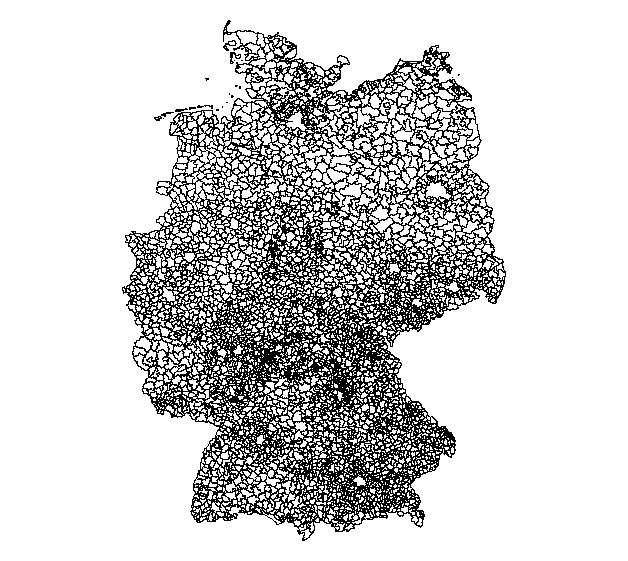
\includegraphics{D:/GitHub/IntroR/buildingblocks/figure/DEU3.png}

\end{frame}

\begin{frame}[fragile]{Gemeinden in Deutschland}
\protect\hypertarget{gemeinden-in-deutschland}{}

\href{http://www.geodatenzentrum.de/geodaten/gdz_rahmen.gdz_div?gdz_spr=deu\&gdz_akt_zeile=5\&gdz_anz_zeile=1\&gdz_unt_zeile=15\&gdz_user_id=0}{Bundesamt
für Kartographie und Geodäsie (BKG)}

\begin{Shaded}
\begin{Highlighting}[]
\NormalTok{krs <-}\StringTok{ }\NormalTok{maptools}\OperatorTok{::}\KeywordTok{readShapePoly}\NormalTok{(}\StringTok{"vg250_krs.shp"}\NormalTok{)}
\KeywordTok{plot}\NormalTok{(krs)}
\end{Highlighting}
\end{Shaded}

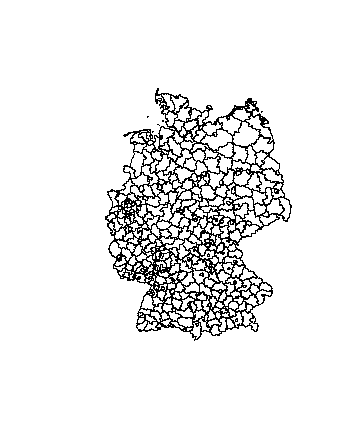
\includegraphics{D:/GitHub/IntroR/buildingblocks/figure/vg250_krs.png}

\end{frame}

\begin{frame}[fragile]{Aufgabe: Download von Shapefiles für die
Gemeinden Deutschlands}
\protect\hypertarget{aufgabe-download-von-shapefiles-fur-die-gemeinden-deutschlands}{}

\begin{itemize}
\tightlist
\item
  Lade die Shapefiles Datei (UTM32 Kompakt) von
  \href{http://www.geodatenzentrum.de/geodaten/gdz_rahmen.gdz_div?gdz_spr=deu\&gdz_akt_zeile=5\&gdz_anz_zeile=1\&gdz_unt_zeile=15\&gdz_user_id=0}{\textbf{hier}}
  herunter.
\item
  Entpacke den zip-Ordner und importiere den Shapefile
  (\texttt{VG250\_F.shp}) mit den Gemeinden, mit einer geeigneten
  Funktion.
\end{itemize}

\end{frame}

\begin{frame}[fragile]{Kreise eines Bundeslandes}
\protect\hypertarget{kreise-eines-bundeslandes}{}

\begin{Shaded}
\begin{Highlighting}[]
\NormalTok{fds <-}\StringTok{ }\KeywordTok{substr}\NormalTok{(krs}\OperatorTok{@}\NormalTok{data}\OperatorTok{$}\NormalTok{AGS,}\DecValTok{1}\NormalTok{,}\DecValTok{2}\NormalTok{)}
\KeywordTok{plot}\NormalTok{(krs[fds}\OperatorTok{==}\StringTok{"05"}\NormalTok{,])}
\end{Highlighting}
\end{Shaded}

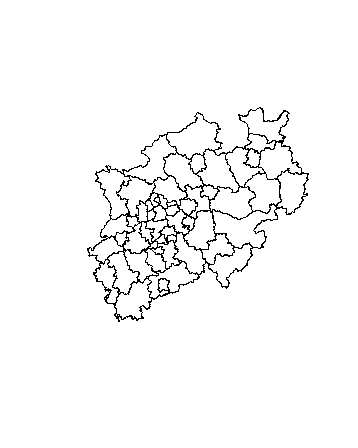
\includegraphics{D:/GitHub/IntroR/buildingblocks/figure/KreiseNRW.png}

\end{frame}

\begin{frame}{A6B Aufgabe: Eine Karte für das Saarland erzeugen}
\protect\hypertarget{a6b-aufgabe-eine-karte-fur-das-saarland-erzeugen}{}

\begin{itemize}
\item
  Schränke die Daten auf das Saarland ein, und zeichne eine Karte vom
  Saarland.
\item
  Speichere den Datensatz in geeigneter Form ab.
\end{itemize}

\end{frame}

\begin{frame}[fragile]{Andere Quellen}
\protect\hypertarget{andere-quellen}{}

\begin{itemize}
\tightlist
\item
  \href{http://msi.nga.mil/NGAPortal/MSI.portal?_nfpb=true\&_pageLabel=msi_portal_page_62\&pubCode=0015}{\textbf{World
  Port Index}}
\end{itemize}

\begin{Shaded}
\begin{Highlighting}[]
\KeywordTok{library}\NormalTok{(rgdal)}
\NormalTok{WPI <-}\StringTok{ }\KeywordTok{readOGR}\NormalTok{ (}\StringTok{"WPI.shp"}\NormalTok{,}\StringTok{"WPI"}\NormalTok{)}
\KeywordTok{plot}\NormalTok{(WPI)}
\end{Highlighting}
\end{Shaded}


\includegraphics{D:/GitHub/IntroR/buildingblocks/figure/WPI.png}

Datenbanken für Karten

\begin{Shaded}
\begin{Highlighting}[]
\KeywordTok{library}\NormalTok{(mapdata)}
\end{Highlighting}
\end{Shaded}

\end{frame}

\begin{frame}[fragile]{Das Paket \texttt{maps} - Mehr Information}
\protect\hypertarget{das-paket-maps---mehr-information}{}

\begin{itemize}
\tightlist
\item
  Nur für manche Staaten bekommt man mit dem Paket \texttt{maps}
  Umkreise für Einheiten unterhalb der Staatsgrenze (bspw. Frankreich,
  USA).
\end{itemize}

\begin{Shaded}
\begin{Highlighting}[]
\KeywordTok{library}\NormalTok{(maps)}
\KeywordTok{data}\NormalTok{(world.cities)}
\KeywordTok{map}\NormalTok{(}\StringTok{"france"}\NormalTok{)}
\KeywordTok{map.cities}\NormalTok{(world.cities,}\DataTypeTok{col=}\StringTok{"blue"}\NormalTok{)}
\end{Highlighting}
\end{Shaded}


\includegraphics{shapefiles_files/figure-beamer/unnamed-chunk-44-1.pdf}

\end{frame}

\begin{frame}[fragile]{Das Rstudio Addin \texttt{colourpicker}}
\protect\hypertarget{das-rstudio-addin-colourpicker}{}

\begin{Shaded}
\begin{Highlighting}[]
\KeywordTok{install.packages}\NormalTok{(}\StringTok{"colourpicker"}\NormalTok{)}
\end{Highlighting}
\end{Shaded}

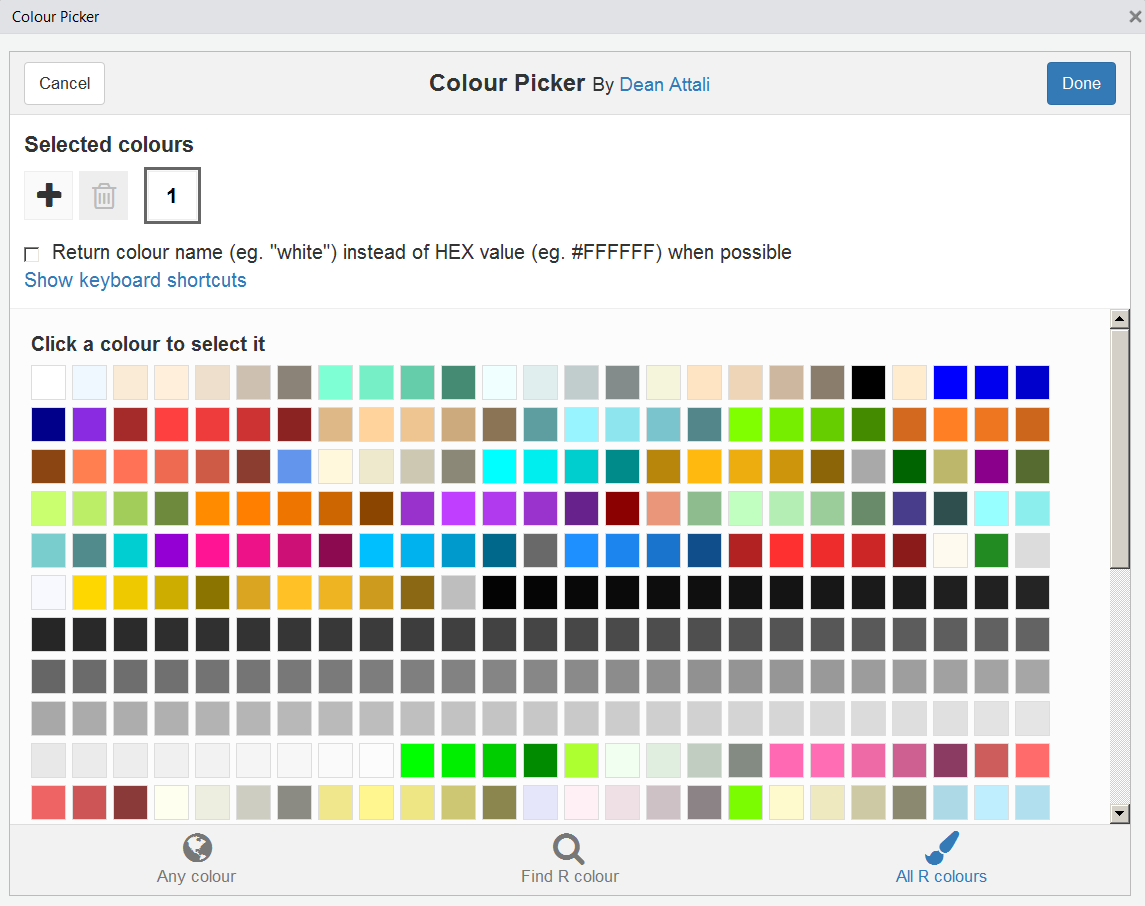
\includegraphics{D:/GitHub/IntroR/buildingblocks/figure/colourpicker.PNG}

\end{frame}

\begin{frame}{Weitere Quelle -
\href{https://www.bundeswahlleiter.de/bundestagswahlen/2017/wahlkreiseinteilung/downloads.html}{Shapefiles
für Wahlkreise}}
\protect\hypertarget{weitere-quelle---shapefiles-fur-wahlkreise}{}


\includegraphics{D:/GitHub/IntroR/buildingblocks/figure/shapefiles_btw.PNG}

\end{frame}

\begin{frame}{\href{http://ec.europa.eu/eurostat/de/web/gisco/geodata/reference-data/administrative-units-statistical-units}{Shapefiles
bei Eurostat}}
\protect\hypertarget{shapefiles-bei-eurostat}{}

\begin{itemize}
\tightlist
\item
  \href{http://epp.eurostat.ec.europa.eu/portal/page/portal/gisco_Geographical_information_maps/popups/\%20references/administrative_units_statistical_units_1}{\textbf{Eurostat
  Karten}} - in der Regel die Europäischen Mitgliedsstaaten
\end{itemize}

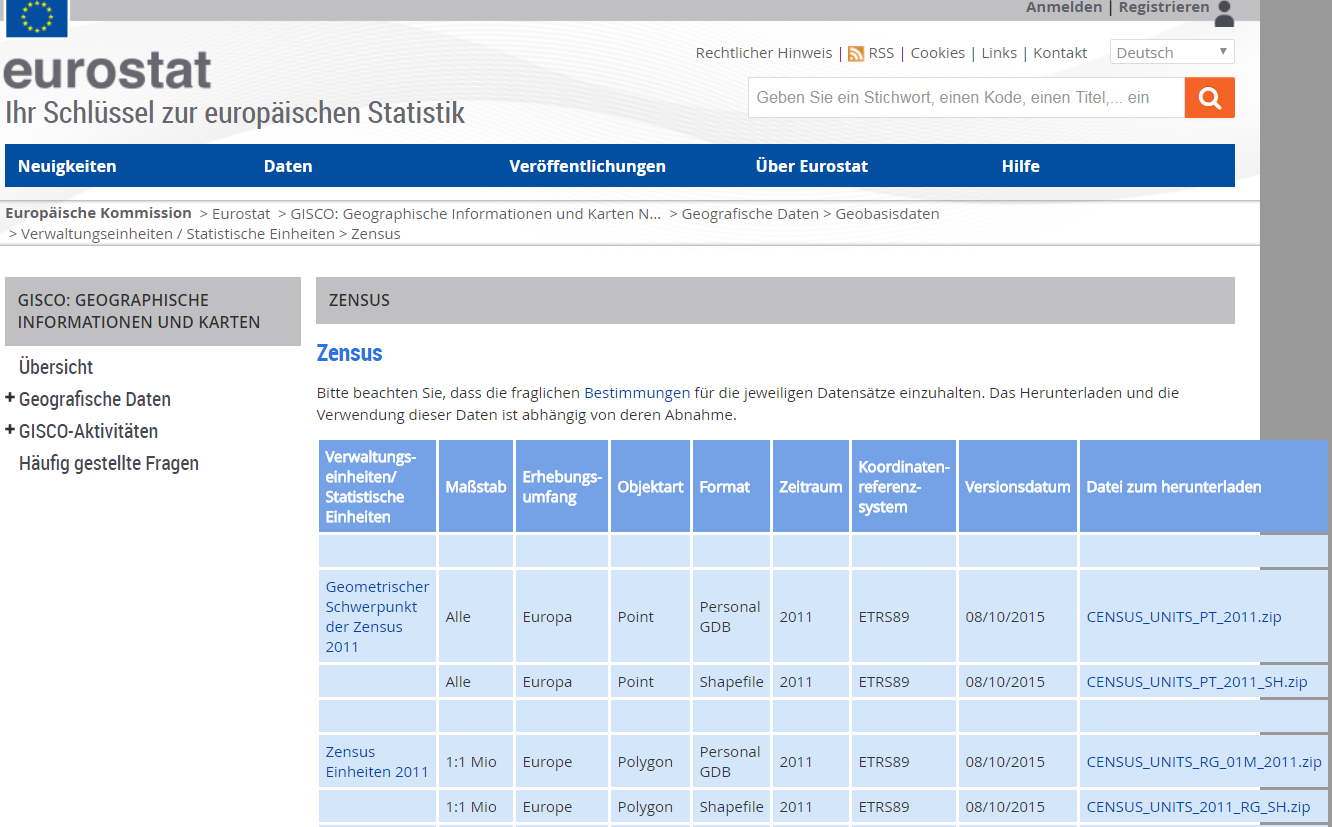
\includegraphics{D:/GitHub/IntroR/buildingblocks/figure/Eurostat_Zensus.PNG}

\end{frame}

\begin{frame}{Weitere Quellen für Shapefiles}
\protect\hypertarget{weitere-quellen-fur-shapefiles}{}

\begin{itemize}
\tightlist
\item
  \href{https://www.ordnancesurvey.co.uk/business-and-government/products/opendata-products-grid.html}{\textbf{Open
  linked data}} - Ordnance Survey (GB)
\end{itemize}

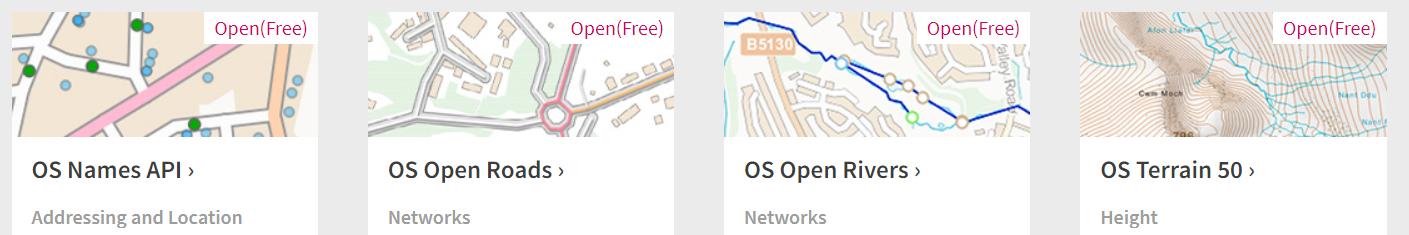
\includegraphics{D:/GitHub/IntroR/buildingblocks/figure/OpenLinkedData.PNG}

\begin{itemize}
\item
  \href{http://thematicmapping.org/downloads/world_borders.php}{\textbf{World
  Borders Datensatz}}
\item
  \href{https://www.nhgis.org/}{\textbf{National Historical Information
  System}}
\item
  \href{http://www.freemapdata.com/html/free_polygon_data.html}{\textbf{Freie
  Polygon-Daten für die USA}}
\item
  Überblick über -
  \href{https://science.nature.nps.gov/im/datamgmt/statistics/r/advanced/spatial.cfm}{\textbf{Spatial
  Data in R}}
\end{itemize}

\end{frame}

\end{document}
